\documentclass[11pt,oribibl]{llncs}

\usepackage[dvips]{graphicx}
\usepackage{pstricks}
\usepackage{rotating}
\usepackage{multirow}
\usepackage{amsmath}
\usepackage{amssymb}

\title{A Viewpoint-Based Framework for Discussing the Use of Multiple Modelling Representations}
\author{Nigel Stanger}
\institute{University of Otago, Dunedin, New Zealand \\ \email{nstanger@infoscience.otago.ac.nz}}

% misc shortcuts
\newcommand{\ER}{\mathit{E\textrm{-}R}}
\newcommand{\Martin}{\mathit{ERD_{Martin}}}
\newcommand{\Chen}{\mathit{ERD_{Chen}}}
\newcommand{\FD}{\mathit{FuncDep}}
\newcommand{\Smith}{\mathit{FDD_{Smith}}}
\newcommand{\RM}{\mathit{Relational}}
\newcommand{\SQL}{\mathit{SQL/92}}
\newcommand{\DF}{\mathit{DataFlow}}
\newcommand{\Gane}{\mathit{DFD_{G\&S}}}
\newcommand{\UsedCars}{V_{\mathit{cars}}}

\begin{document}

\maketitle

\begin{abstract}
When modelling a real-world phenomenon, it can often be useful to have multiple descriptions of the phenomenon, each expressed using a different modelling approach or \emph{representation}. Different representations such as entity-relationship modelling, data flow modelling and use case modelling allow analysts to describe different aspects of real-world phenomena, thus providing a more thorough understanding than if a single representation were used. Researchers working with multiple representations have approached the problem from many different fields, resulting in a diverse and potentially confusing set of terminologies. In this paper is described a viewpoint-based framework for discussing the use of multiple modelling representations to describe real-world phenomena. This framework provides a consistent and integrated terminology for researchers working with multiple representations. An abstract notation is also defined for expressing concepts within the framework.
\end{abstract}

%================================================================================

\section{Introduction}
\label{Sec:Introduction}

In this paper is described a framework for discussing the use of multiple modelling approaches or \emph{representations} to describe a real-world phenomenon. This framework is derived from work on \emph{viewpoint-oriented design}, and provides a consistent and integrated terminology for researchers working with multiple modelling representations. An abstract notation for expressing various concepts within the framework is also defined.

Why is it useful to describe the same phenomenon using multiple modelling representations? There are several reasons, such the ability to provide a more complete description of the phenomenon in question, and because some representations are better suited to particular problems than others. The use of multiple representations and associated issues are discussed in Sect.~\ref{Sec:MultipleRepresentations}.

The framework described in this paper is primarily derived from earlier work in the area of viewpoint-oriented design methods. The basic concepts of viewpoint-oriented design methods are introduced in Sect.~\ref{Sec:Viewpoints}, and a lack of clarity is identified with respect to the definitions of some fundamental concepts (in particular, the meaning of the term `representation').

The author's framework arose out of the need to clarify the definitions of various terms and also to integrate and simplify the potentially confusing range of terminologies developed by other authors. The framework is discussed in Sect.~\ref{Sec:Framework}. In particular, the terms `representation', `technique' and `scheme' are clarified, and the new terms `description', `construct' and `element' are defined.

The author has also developed an abstract notation for expressing various framework concepts in a concise manner. This notation is defined in Sect.~\ref{Sec:Notation}.

The paper is concluded in Sect.~\ref{Sec:Conclusion}.

%================================================================================

\section{Using multiple representations to describe a phenomenon}
\label{Sec:MultipleRepresentations}

There are many different types of information to be considered when designing an information system, and a wide variety of modelling approaches and notations have been developed to capture these different types of information: entity-relationship diagrams (ERDs), data flow diagrams (DFDs), use case diagrams, the relational model, formal methods and so on. Problems can arise when useful information is omitted from a design. Consider an information system whose data structures are designed using entity-relationship diagrams and are implemented in a relational database. Data entry forms derived from these models are built using a rapid application development tool. Good design practices are followed throughout, yet the finished application is difficult to use. Some of the commonly used data entry forms have multiple states, but the transitions between these states are unclear to users because state information was not included in the system design.

While this is a purely theoretical example, it serves to illustrate an important point. Information systems are typically built to handle the data processing requirements of some real-world phenomenon. Such real-world phenomena may often be too complex to describe using a single modelling approach, or \emph{representation}. This is supported by the plethora of different representations that currently exist \cite{Hull:R:1987,Tsic:D:1982}, including those that model the structure of data (such as entity-relationship modelling), and those that model how data move around a system (such as data flow diagrams). This implies that in order to completely model a phenomenon, multiple descriptions of the phenomenon are required, expressed using different representations.

Using multiple representations to describe a phenomenon is also important in other ways:
\begin{itemize}
	\item If multiple developers are working on a project, each may prefer or be required to use a different representation to describe their particular part of the project \cite{Atze:P:1996:EDBT}. Meyers \cite{Meye:S:1991:IEEE} also notes that it can be very useful to simultaneously view a system in several different ways when multiple people are working on the system.
	\item Particular subproblems may be better described using some representations than others \cite{East:SM:1991:PhD}.
	\item Multiple representations are important when integrating heterogeneous data sources to form a federated or distributed system \cite{Atze:P:1996:EDBT}, as each data source may potentially use a different logical data model.
\end{itemize}

The idea of using multiple representations to model a phenomenon is not new. Grundy et al. have been examining the issues associated with building multi-view editing systems and integrated software development environments for many years \cite{Grun:JC:1993:PhD,Grun:JC:1997:IJAST,Grun:JC:1995:CAiSE}, with emphasis on the issue of maintaining consistency between different views or descriptions of the same phenomenon \cite{Grun:JC:1996:SPE,Hosk:JG:1995:NZCS}. Grundy's work was derived from earlier work on multi-view editing systems for software engineering, such as FIELD \cite{Reis:SP:1990:IEEE} and Zeus \cite{Brow:MH:1992:Zeus}.

Atzeni and Torlone \cite{Atze:P:1997:MDM} suggested the idea of translating between different representations as a means of facilitating the use of multiple representations. They proposed a formal model based on lattice theory \cite{Atze:P:1995:Lattice} that allowed them to express many different data modelling approaches using primitive constructs of a single underlying representation.

Su et al. \cite{Su:SYW:1993,Su:SYW:1992} approached the use of multiple representations from the point of view of integrating heterogeneous data sources in order to build federated and distributed databases. Their approach is similar in many respects to that taken by Atzeni and Torlone, except that the underlying representation is object-oriented rather than mathematically based.

All three groups developed their work independently of each other over a similar time period (1991--94), and each approached the use of multiple modelling representations from a different starting point. This has resulted in a diverse and potentially confusing set of terminologies (see Table~\ref{Tab.MultipleRepresentations.Terminology}). A single integrated terminology would reduce this potential for confusion.

%%%%%%%%%%%%%%%%%%%%%%%%%%%%%%%

% table notes
\newcommand{\tabnote}[1]{\textrm{\textsuperscript{#1}}}
\newcounter{tnote}
\renewcommand{\thetnote}{\alph{tnote}}
\newenvironment{tabnotes}[1]%
	{	\vspace{\baselineskip}
		\begin{minipage}{0.95\columnwidth}
			\textbf{#1}
			\begin{list}{\thetnote}%
			{	\setlength{\topsep}{0pt}
				\setlength{\itemsep}{0pt}
				\setlength{\parsep}{0pt}
				\usecounter{tnote}
				\renewcommand{\makelabel}[1]{\hfil{\textsuperscript{##1}}}
			}
	}%
	{		\end{list}
		\end{minipage}
	}

% a few lengths to use in \multirow commands
\newlength{\mra}
\newlength{\mrb}
\newlength{\mrc}
\newlength{\mrd}
\newlength{\mre}

% humongous `}'s for use in tables
\newlength{\BIGlen}
\newcommand{\BIGL}[2][0cm]{
	\setlength{\BIGlen}{#1} \divide\BIGlen by 2
	$\left\}\text{ \rule[-\BIGlen]{0cm}{#1}#2}\right.$}

\begin{sidewaystable}[p]
	\centering
	\caption{Comparison of viewpoint/representation terminologies}
	\label{Tab.MultipleRepresentations.Terminology}
	\scriptsize
	\settowidth{\mra}{specification}
	\settowidth{\mrb}{\textbf{Torlone [3]}}
	\settowidth{\mrc}{\BIGL[3.1cm]{\shortstack{data \\ model}}}
	\settowidth{\mrd}{~relational model~}
	\settowidth{\mre}{\textbf{Easterbrook}}
	\medskip\hrule\smallskip
	\begin{tabular}{cp{3.7cm}ccccccc}
																							&																										&																			&	\multicolumn{6}{c}{\textbf{Corresponding term used by:}}	\\
		\cline{4-9}
		\textbf{Term used}																	&																										&																			&	\textbf{Finkelstein}															&	\textbf{Easterbrook}								&	\textbf{Darke \&}					&	\textbf{Grundy}										&	\textbf{Atzeni \&}									&	\textbf{Su \emph{et al.}}	\\
		\textbf{by the author}																&	\textbf{Meaning}																					&	\textbf{Example}														&	\textbf{\cite{Fink:ACW:1989}}													&	\textbf{\cite{East:SM:1991:PhD}}					&	\textbf{Shanks \cite{Dark:P:1995}}	&	\textbf{\emph{et al.} \cite{Grun:JC:1997:IJAST}}	&	\textbf{Torlone \cite{Atze:P:1997:MDM}}				&	\textbf{\cite{Su:SYW:1992}}	\\
		\\
		perspective																			&	A description of a real-world pheno\-menon that has internal consistency and an identifiable focus.	&	--																		&	--																				&	perspective											&	perspective							&	--													&	--													&	--	\\
		\\
		viewpoint																			&	The formatted description of a perspective.															&	--																		&	ViewPoint																		&	viewpoint											&	viewpoint							&	--													&	--													&	--	\\
		\\
		technique																			&	A collection of abstract constructs that form a modelling `method'.									&	~relational model~														&	\multirow{10}{\mra}{\centering \BIGL[3.1cm]{style}}								&	\multirow{10}{\mre}{\centering \BIGL[3.1cm]{style}}	&	technique							&	--													&	\multirow{10}{\mrb}{\centering \BIGL[3.1cm]{model}}	&	\multirow{10}{\mrc}{\centering \BIGL[3.1cm]{\shortstack{data \\ model}}}	\\
		\\
		scheme																				&	A collection of concrete constructs that form a modelling `notation'.								&	SQL/92																	&																					&														&	scheme								&	--	\\
		\\
		representation																		&	The combination of a particular technique and scheme.												&	\multicolumn{1}{p{\mrd}}{\centering relational model +~SQL/92}			&																					&														&	representation						&	representation	\\
		\\
		description																			&	An instantiation of a representation.																&	SQL/92 schema															&	specification																	&	description											&	--									&	view												&	scheme												&	schema	\\
		\\
		construct																			&	The basic unit of a representation.																	&	a relation																&	--																				&	--													&	--									&	--													&	construct											&	class\tabnote{\ref{TermD}}	\\
		\\
		element																				&	An instantiation of a construct within a particular description.									&	\textsf{Staff} table													&	--																				&	--													&	--									&	component											&	varies\tabnote{\ref{TermA}}							&	object	\\
	\end{tabular}

	\begin{tabnotes}{Notes on Table~\ref{Tab.MultipleRepresentations.Terminology}:}
		\item\label{TermD} Also `construct'.
		\item\label{TermA} Terms used include `component', `element' and `concept'.
		\item[]	`--' indicates that a term is not used by that author.
	\end{tabnotes}
	\smallskip\hrule
\end{sidewaystable}

%%%%%%%%%%%%%%%%%%%%%%%%%%%%%%%

In addition to the three groups outlined above, viewpoint researchers first suggested using multiple representations to describe viewpoints over a decade ago \cite{Fink:ACW:1989}. A viewpoint is effectively a formalisation of the perceptions of stakeholders with respect to some real-world phenomenon. Since we are dealing with the use of multiple representations to describe real-world phenomena, viewpoints should provide a useful framework within which to discuss such use \cite{Stan:N:1997:ECIS97}. The author's framework will be described in Sect.~\ref{Sec:Framework}, but first the basic concepts of viewpoint-oriented methods must be defined.

%================================================================================

\section{Viewpoint concepts}
\label{Sec:Viewpoints}

A \emph{viewpoint} can be thought of as a formalisation of the perceptions of a stakeholder group with respect to some real-world phenomenon that is being modelled. The first viewpoint-oriented approach (Mullery's CORE method) was introduced in 1979 \cite{Mull:G:1979}, but the concept of a viewpoint was not formalised until ten years later \cite{Fink:ACW:1989}.

Viewpoint-oriented methods were originally developed to assist with requirements definition in a software engineering environment \cite{Mull:G:1979}, and subsequent research has followed a similar direction \cite{East:SM:1991:PhD,East:SM:1996,Koto:G:1996,Nuse:B:1994}. The focus of the author's research has been on how to facilitate the use of multiple representations to describe a single viewpoint \cite{Stan:N:1999:PhD,Stan:N:1997:ECIS97}.

In Fig.~\ref{Fig.Background.Terminology} are shown the relationships between the concepts of view\-point-oriented methods. This initial framework was derived by the author \cite{Stan:N:1997:ECIS97} from the work of Finkelstein et al. \cite{Fink:ACW:1989}, Easterbrook \cite{East:SM:1991:PhD} and Darke and Shanks \cite{Dark:P:1995}. Their terminologies are also summarised in Table~\ref{Tab.MultipleRepresentations.Terminology}.

%%%%%%%%%%%%%%%%%%%%

\begin{figure}[htb]
	\centering
	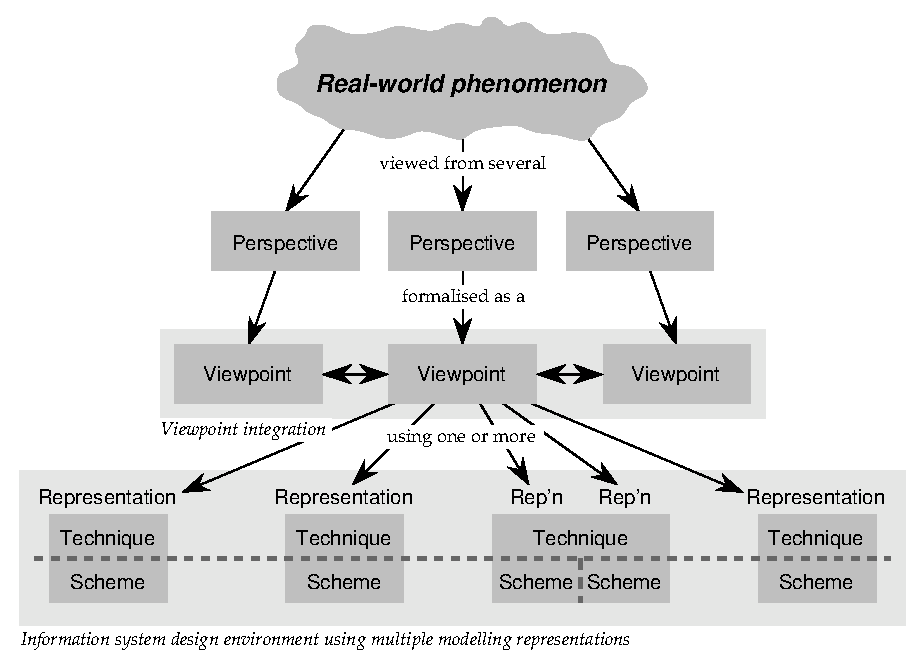
\includegraphics[width=0.95\columnwidth,keepaspectratio]{Terminology}
	\caption{Relationship between perspectives, viewpoints and representations}
	\label{Fig.Background.Terminology}
\end{figure}

%%%%%%%%%%%%%%%%%%%%

%================================================================================

\subsection{Perspectives and viewpoints}
\label{Sec:Background:Viewpoints:Perspectives}

Easterbrook \cite{East:SM:1991:PhD} defines a \emph{perspective} as ``a description of an area of knowledge which has internal consistency and an identifiable focus of attention''. During the requirements definition phase of systems analysis, developers may encounter many different perspectives on the problem being modelled. Perspectives may overlap and/or conflict with each other in various ways.

Finkelstein et al. \cite{Fink:ACW:1989} describe a \emph{viewpoint} as comprising the following parts:
\begin{itemize}
	\item ``a \emph{style}, the representation scheme in which the ViewPoint [\emph{sic}] expresses what it can see (examples of styles are data flow analysis, entity-relationship-attribute modelling, Petri nets, equational logic, and so on);
	\item a \emph{domain} defines which part of the `world' delineated in the style (given that the style defines a structured representation) can be seen by the ViewPoint (for example, a lift-control system would include domains such as user, lift and controller);
	\item a \emph{specification}, the statements expressed in the ViewPoint's style describing particular domains;
	\item a \emph{work plan}, how and in what circumstances the contents of the specification can be changed; [and]
	\item a \emph{work record}, an account of the current state of the development.''
\end{itemize}

Easterbrook \cite{East:SM:1991:PhD} simplifies this description by defining a viewpoint as ``the formatted representation of a perspective'', and notes that a perspective is a ``more abstract version of a viewpoint''. In effect, a viewpoint is the formalisation of a particular perspective, so there is a one-to-one correspondence between a viewpoint and the perspective it formalises, as illustrated in Fig.~\ref{Fig.Background.Terminology}.

The term `viewpoint' is very similar to the term `view' as used in multi-view editing systems \cite{Brow:MH:1992:Zeus,Grun:JC:1993:PhD,Jaco:DA:1995:MultiView,Meye:S:1991:IEEE}. These terms refer to different concepts, however: a `view' is more akin to the concept of a \emph{description}, which will be introduced in Sect.~\ref{Sec:Framework}. The similarity of the two terms has led to some confusion: the terms `viewpoint' and `view' have been used interchangeably in the past \cite{Jaco:DA:1995:MultiView}. 

Darke and Shanks \cite{Dark:P:1995} define two main types of viewpoint:
\begin{enumerate}
	\item \emph{user viewpoints} that capture ``the perceptions and domain knowledge of a particular user group, reflecting the particular portion of the application domain relevant to that group''; and
	\item \emph{developer viewpoints} that capture ``the perceptions, domain knowledge and modelling perspective relevant to a systems analyst or other developer responsible for producing some component of the requirements specification''.
\end{enumerate}

Since a viewpoint is the formalisation of a perspective, some form of model is required to provide the formalised structure. The concept of a \emph{representation} provides this.

%================================================================================

\subsection{Representations}
\label{Sec:Background:Viewpoints:Representations}

Darke and Shanks \cite{Dark:P:1994:WP21/94} note that viewpoints may be described using different representation \emph{techniques}, within each of which there may be available a number of representation \emph{schemes}. Neither Darke and Shanks nor Finkelstein et al. \cite{Fink:ACW:1989} clearly define the terms `representation', `technique' or `scheme'; rather, they introduce each term by means of examples. This has led to some confusion in the use of this terminology. Darke and Shanks use the terms `representation' and `representation technique' interchangeably, while Finkelstein et al., as can be seen in their definition of a `style', use the term `representation scheme' in a similar way.

The intent appears to be that a \emph{representation} should be thought of as a structured modelling approach that can be used to describe the content of a viewpoint. In order to clarify the confusion in terminology, the author has refined this informal definition and defined a representation as the combination of a particular technique and scheme to describe a viewpoint. This will be discussed further in Sect.~\ref{Sec:Framework}.

Darke and Shanks \cite{Dark:P:1995} group representations into three general categories:
\begin{enumerate}
	\item \emph{informal} representations that form unstructured descriptions, often expressed using natural language or simple diagrams;
	\item \emph{semi-formal} representations that form structured descriptions, such as entity-re\-la\-tion\-ship modelling or data flow diagrams; and
	\item \emph{formal} representations that form structured descriptions and include a set of operators for processing these descriptions, such as the relational model or logic-based models.
\end{enumerate}

Unlike informal representations, which are often ill-defined, inconsistent and ambiguous, semi-formal and formal representations are well-defined, consistent and generally unambiguous. A key feature of formal representations that is lacking in semi-formal representations is the inclusion of operators that allow assertions to be made about the viewpoints being described; Greenspan et al. \cite{Gree:S:1994:RML} describe this as the ability to `reason' about representations. User viewpoints are typically defined using informal representations, whereas developer viewpoints are typically defined using semi-formal or formal representations.

Finkelstein et al. \cite{Fink:ACW:1989} first mooted the idea of using multiple representations to describe a viewpoint in 1989, but there has been surprisingly little work in this area since then. Darke and Shanks \cite{Dark:P:1996:RE} found in a review of twelve different viewpoint development approaches that only two supported multiple representations to describe a single viewpoint: the Soft Systems methodology \cite{Chec:PB:1981:SSM} and Scenario Analysis \cite{Hsia:P:1994:Scenario}, both of which are user viewpoint approaches rather than developer viewpoint approaches.

The author's own research \cite{Stan:N:1999:PhD,Stan:N:1997:ECIS97} has followed the approach of using multiple representations to describe a single \emph{developer} viewpoint, and uses an integrated terminology framework derived from viewpoint-oriented methods. This framework will now be described.

%================================================================================

\section{The viewpoint framework for discussing the use of multiple modelling representations}
\label{Sec:Framework}

Looking at Table~\ref{Tab.MultipleRepresentations.Terminology}, there is an obvious dichotomy between the three viewpoint terminologies on the left and the three multiple-view terminologies on the right. The viewpoint terminologies deal primarily with `high level' concepts and ignore how representations are internally structured; conversely, the multiple-view terminologies deal primarily with constructs within representations and ignore higher-level structure. The two sets of terminology are clearly related, yet the only real overlap between them is at the representation level.

There are also many synonyms in the terminologies presented in Table~\ref{Tab.MultipleRepresentations.Terminology}, for example, the terms `style', `representation', `model' and `data model' are all used to refer to similar concepts. Conversely, the term `scheme' is used to refer to two completely different concepts. Such variation can lead to confusion, so there is a definite need to develop a consistent and integrated terminology framework.

The initial framework shown in Fig.~\ref{Fig.Background.Terminology} provides a good basis for extension, but the author has identified some confusion over the exact definitions of the terms `representation', `technique' and `scheme'. The author has addressed this confusion by clearly defining these terms, and has extended the original framework with the concepts of \emph{descriptions}, \emph{constructs} of representations and \emph{elements} of descriptions (see Fig.~\ref{Fig.MultipleRepresentations.Terminology}).

%%%%%%%%%%%%%%%%%%%%

\begin{figure}[htbp]
	\centering
	\psset{unit=0.8cm}
	\begin{pspicture}(15,15.35)
		\rput[bl](0,0){\includegraphics[width=12cm,keepaspectratio]%
		                               {Terminology2}}
		\rput(2.55,6.75){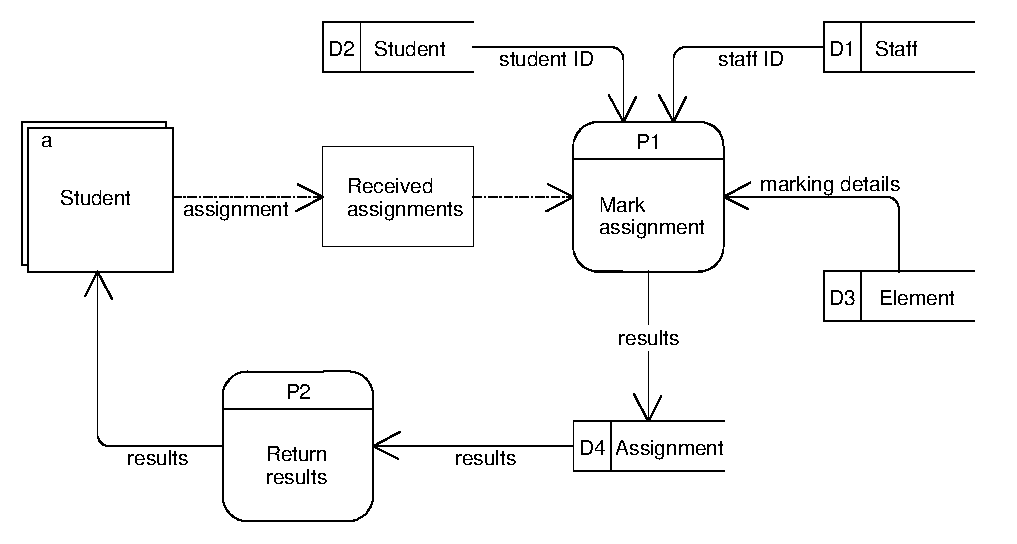
\includegraphics[width=2cm,keepaspectratio]{MarksDFD}}
		\rput(6,6.75){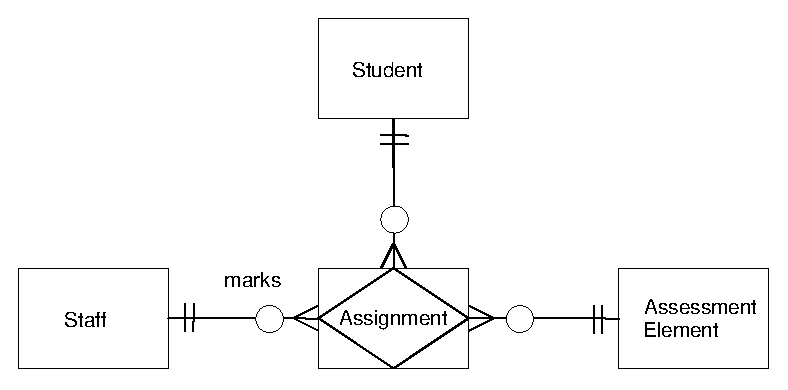
\includegraphics[width=2cm,keepaspectratio]{MarksERD}}
		\rput(12.95,6.75){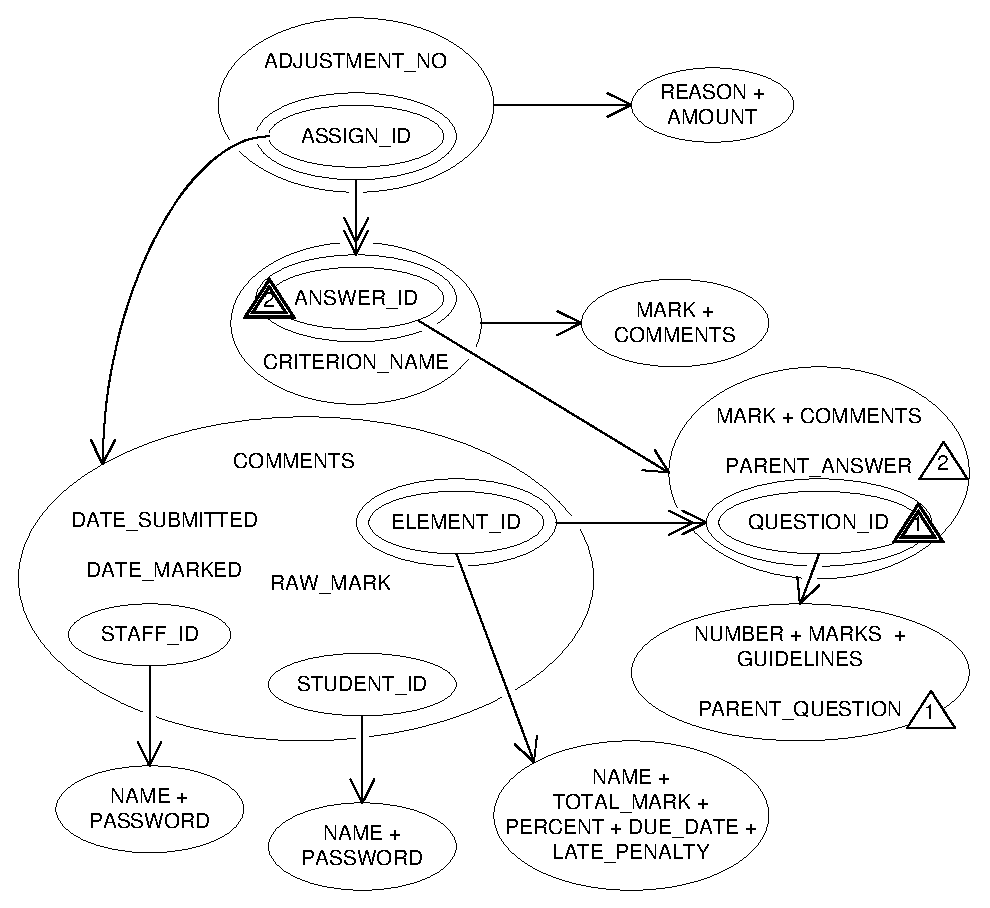
\includegraphics[width=2cm,keepaspectratio]{MarksFDD}}
	\end{pspicture}
	\caption{The extended terminology framework}
	\label{Fig.MultipleRepresentations.Terminology}
\end{figure}

%%%%%%%%%%%%%%%%%%%%

%================================================================================

\subsection{Representations}
\label{Sec:MultipleRepresentations:Representations:Representations}

Informally, a data modelling representation can be thought of as comprising two main parts:
\begin{enumerate}
	\item a \emph{generic} part that specifies the generic constructs that may be used to describe a viewpoint, such as entities, relations, and so on; which then determines
	\item a \emph{specialised} part that specifies the constructs peculiar to the representation, along with their visual appearance or notation, such as boxes for entities, SQL \texttt{CREATE TABLE} statements for relations, and so on.
\end{enumerate}

Finkelstein et al.'s \cite{Fink:ACW:1989} use of the term `style' does not clearly distinguish between these two parts; conversely, the `techniques' and `schemes' of Darke and Shanks \cite{Dark:P:1994:WP21/94} match these two parts well. It is therefore proposed to use the term \emph{technique} to refer to the generic part of a representation, and the term \emph{scheme} to refer to the specialised part of a representation. In practical terms, a technique can be thought of as a modelling `approach', such as the entity-relationship approach or the relational model, and a scheme can be thought of as a particular `notation' within that approach, such as a particular entity-relationship notation or relational calculus. Another way to think of this is that a scheme is an `instantiation' of a particular technique.

A \emph{representation} can thus be defined as the combination of a particular technique with a particular scheme, as illustrated in Fig.~\ref{Fig.MultipleRepresentations.Terminology}. In general, a technique may have one or more associated schemes, but each combination of a technique and a scheme forms a distinct representation. For example, the relational model is a technique, with $\mathit{SQL}$ and $\mathit{QUEL}$ as two possible schemes, but the combinations $(\RM,\mathit{SQL})$\footnote{In practice, the many dialects of SQL will form many different representations. This has been ignored here in the interests of clarity.} and $(\RM,\mathit{QUEL})$ form two distinct representations, as shown in Fig.~\ref{Fig.MultipleRepresentations.MultipleSchemes}. Similarly, the entity-relationship approach ($\ER$) is a technique, with $\Martin$ and $\Chen$ as two possible schemes. The combinations $(\ER,\Martin)$ and $(\ER,\Chen)$ again form two distinct representations.

%%%%%%%%%%%%%%%%%%%%

\begin{figure}[htbp]
	\centering
	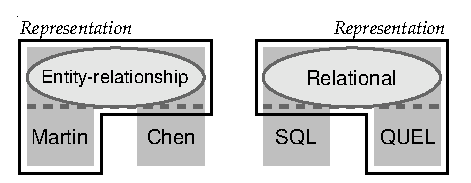
\includegraphics{MultipleSchemes}
	\caption{Multiple schemes within a technique}
	\label{Fig.MultipleRepresentations.MultipleSchemes}
\end{figure}

%%%%%%%%%%%%%%%%%%%%

It is expected that a technique will not attempt to specify all possible concepts for all possible schemes within that technique. Rather, a technique defines the `base' model, which is then specialised and extended by schemes to form a representation. This implies that a scheme may provide new constructs to a representation that have no direct analogue in the technique. For example, the relational technique \cite{Codd:EF:1970} does not include general constraints, but they are an important feature of the relational scheme SQL/92 \cite{Date:CJ:1997:SQL}. Similarly, type hierarchies are not part of the base E-R technique \cite{Chen:PP:1976}, but they do appear in some E-R schemes.

%================================================================================

\subsection{Descriptions}
\label{Sec:MultipleRepresentations:Representations:Descriptions}

Representations are an abstract concept, so they must be instantiated in some way in order to describe the content of a viewpoint. One way to view the instantiation of a representation is as a set of `statements' that describe a viewpoint or some subset thereof. Finkelstein et al. \cite{Fink:ACW:1989} refer to this as a `specification' or `description'; Easterbrook \cite{East:SM:1991:PhD} also refers to this concept as a description. The author has adopted the term `description' as it emphasises the idea that they are used to \emph{describe} a viewpoint.

A viewpoint is thus specified by a set of \emph{descriptions}, each expressed using some representation, as shown in Fig.~\ref{Fig.MultipleRepresentations.Terminology}. Each description may describe either the whole viewpoint or some subset of the viewpoint; this is analogous to the concept of a `view' as used in multi-view editing systems \cite{Brow:MH:1992:Zeus,Grun:JC:1993:PhD,Jaco:DA:1995:MultiView,Meye:S:1991:IEEE}. For example, a developer viewpoint might be specified by union of the following four descriptions:

\begin{enumerate}
	\item an object class description expressed using Unified Modelling Language (UML) class diagram notation \cite{Mull:PA:1997:UML};
	\item a functional dependency description expressed using Smith functional dependency diagram notation \cite{Smit:HC:1985,Stan:N:1999:Smith};
	\item a relational description expressed using SQL/92; and
	\item a data flow description expressed using Gane \&~Sarson data flow diagram notation \cite{Gane:C:1979}.
\end{enumerate}

Similarly, a user viewpoint might be specified by the union of a natural language description and a collection of diagrammatic descriptions. Descriptions may be distinct from each other, or they may overlap in a manner similar to viewpoints. Such redundancy can be useful in exposing conflicts both between descriptions and between viewpoints \cite{East:SM:1991:PhD}.

%================================================================================

\subsection{Constructs and elements}
\label{Sec:MultipleRepresentations:Representations:Constructs}

Every representation comprises a collection of \emph{constructs}. These may be divided into generic constructs associated with the technique (\emph{technique-level constructs}) and specialised constructs associated with the scheme (\emph{scheme-level constructs}), as shown in Fig.~\ref{Fig.MultipleRepresentations.Terminology}. The nature of a construct is defined by its \emph{properties}, which include both its \emph{relationships} with other constructs, and its \emph{attributes}, such as name, domain or cardinality\footnote{The terms `property', `attribute' and `relationship' come from the Object Data Management Group's object model \cite{Catt:RGG:2000:ODMG3}.}. For instance, as illustrated in Fig.~\ref{Fig.MultipleRepresentations.Properties}, a data store in a data flow diagram might have the attributes \emph{name} (the name of the data store), \emph{label} and \emph{fields} (a list of data fields in the data store). The \emph{flows} relationship specifies an association between the data store construct and a list of data flow constructs.

%%%%%%%%%%%%%%%%%%%%

\begin{figure}[htbp]
	\centering
	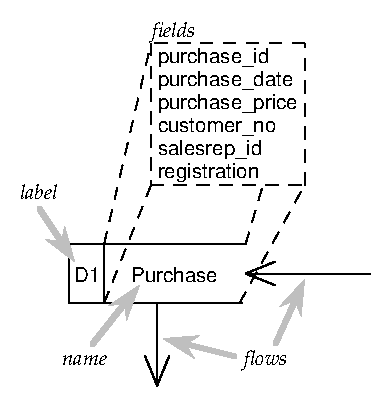
\includegraphics{Properties}
	\caption{Properties of a construct}
	\label{Fig.MultipleRepresentations.Properties}
\end{figure}

%%%%%%%%%%%%%%%%%%%%

In the same way that a description is an instantiation of a representation, an \emph{element} is an instantiation of a construct; elements are combined to build descriptions. Examples of constructs include object classes, processes and attributes; elements corresponding to these constructs could be \textsf{Order}, \textsf{Generate invoice} and \textsf{address}.

%================================================================================

% a representation, i.e., R(T,S); second form has a subscript as second argument
\newcommand{\Representation}[3]{\ensuremath{\mathfrak{#1}(#2,#3)}}
\newcommand{\RepresentationS}[4]{\ensuremath{\mathfrak{#1}_{#2}(#3,#4)}}
\newcommand{\Rep}[1]{\ensuremath{\mathfrak{#1}}}
\newcommand{\RepS}[2]{\ensuremath{\mathfrak{#1}_{#2}}}

% a description, i.e., D(V,T,S)
\newcommand{\Description}[4]{\ensuremath{#1(#2,#3,#4)}}
\newcommand{\rDescription}[5]{\ensuremath{#1(#2,\Representation{#3}{#4}{#5})}}
\newcommand{\rDescriptionS}[6]{\ensuremath{#1(#2,\RepresentationS{#3}{#4}{#5}{#6})}}
\newcommand{\shortDescription}[3]{\ensuremath{#1(#2,\mathfrak{#3})}}
\newcommand{\shortDescriptionS}[4]{\ensuremath{#1(#2,\mathfrak{#3}_{#4})}}

% a construct name
\newcommand{\domain}[1]{\textsc{#1}}

% elements D[e] and D[e:C]
\newcommand{\Element}[2]{\ensuremath{ #1 \left[ #2 \right] }}
\newcommand{\Elementt}[3]{\ensuremath{ #1 \left[ #2 : \domain{#3} \right] }}

% constructs R[C] and R[C:X]; lowercase ones don't have the calligraphic 'R' on front
\newcommand{\construct}[2]{\ensuremath{ #1 \left[ \domain{#2} \right] }}
\newcommand{\Construct}[2]{\ensuremath{ \mathfrak{#1} \left[ \domain{#2} \right] }}

%================================================================================

\section{A notation to express representations, descriptions, constructs and elements}
\label{Sec:Notation}

It can be cumbersome to discuss aspects of representations and descriptions using natural language, for example, `the \textsf{Staff} regular entity element of the description $D_{1}$ (expressed using Martin entity-relationship notation) of the managers' viewpoint'. The author has therefore developed a concise abstract notation for expressing representations, descriptions, constructs of representations and elements of descriptions. This notation is modelled in part on the data transfer notation of Pascoe and Penny \cite{Pasc:RT:1995}. Using the notation, the statement above could be expressed as:
\[	\Elementt{\Description{D_{1}}{V_{mgrs}}{\ER}{\Martin}}{\mathit{staff}}{RegularEntity}\text{.}	\]
The notation is summarised in Table~\ref{Tab.MultipleRepresentations.Notation}. The author has defined additional notations for expressing translations of descriptions from one representation to another \cite{Stan:N:1999:PhD}. For example, the expression:
\[	\Description{D_{1}}{V}{\FD}{\Smith} \rightarrow \Description{D_{2}}{V}{\ER}{\Martin}
\]
denotes the translation within viewpoint $V$ of a functional dependency description $D_{1}$ into an entity-relationship description $D_{2}$. Such additions are beyond the scope of this paper, however; only the base notation is discussed here.

%%%%%%%%%%%%%%%%%%%%%%%%%%%%%%%

\begin{table}[htb]
	\centering
	\caption{Summary of the abstract notation}
	\label{Tab.MultipleRepresentations.Notation}
	\hrule\smallskip
	\begin{tabular}{clp{6.25cm}}
		\textbf{Notation}								&	\textbf{Associated term}	&	\textbf{Definition}	\\
		\\
		$V$												&	Viewpoint					&	A formatted expression of a perspective on a real-world phenomenon.	\\
		\\
		$T$												&	Technique					&	A collection of generic constructs that form a modelling `method', for example, the relational model or object modelling.	\\
		\\
		$S$												&	Scheme						&	A collection of specialised constructs that form a modelling `notation', for example, SQL/92 or UML class diagram notation.	\\
		\\
		\Representation{R}{T}{S} or \Rep{R}				&	Representation				&	Representation \Rep{R} comprises constructs defined by the combination of technique $T$ and scheme $S$.	\\
		\\
		\Description{D}{V}{T}{S} or $D$					&	Description					&	Description $D$ of viewpoint $V$ is expressed using constructs of technique $T$ \& scheme $S$.	\\
		\\
		\construct{\Representation{R}{T}{S}}{con},		&	Construct of a				&	\domain{con} specifies a construct of representation	\\
		\Construct{R}{con}, or \domain{con}				&	representation				&	\Representation{R}{T}{S}.	\\
		\\
		\Elementt{\Description{D}{V}{T}{S}}{e}{con},	&	Element of a				&	$e$ specifies an element (instantiated from con-	\\
		\Elementt{D}{e}{con}, or \Element{D}{e}			&	description					&	struct \domain{con}) of description \Description{D}{V}{T}{S}.	\\
	\end{tabular}
	\smallskip\hrule
\end{table}

%%%%%%%%%%%%%%%%%%%%%%%%%%%%%%%

%================================================================================

\subsection{Description and representation notation}

The notation \Description{D}{V}{T}{S} denotes that description $D$ of viewpoint $V$ is expressed using constructs of technique $T$ and scheme $S$ (this may be abbreviated to $D$ when $V$, $T$ and $S$ are clear). Thus, \Description{D_{1}}{V_{p}}{\ER}{\Martin} denotes a description $D_{1}$ of the viewpoint $V_{p}$ that is expressed using constructs of the entity-relationship technique ($\ER$) and the Martin ERD scheme ($\Martin$) \cite{Mart:J:1990:IE2}.

The notation \Representation{R}{T}{S} denotes a representation \Rep{R} that comprises a collection of constructs defined by the combination of technique $T$ and scheme $S$ (this may be abbreviated to \Rep{R} when $T$ and $S$ are clear). Thus, \RepresentationS{R}{e}{\ER}{\Martin} denotes the representation \RepS{R}{e} formed by combining the constructs of the entity-relationship technique ($\ER$) with the Martin ERD scheme ($\Martin$). This notation is similar to that used by Finkelstein et al. to describe viewpoint styles \cite{Fink:ACW:1989}, but focuses on the technique and scheme used rather than individual constructs within a representation.

The combination of technique $T$ and scheme $S$ forms the representation \Representation{R}{T}{S}, so it is also possible to denote the description \Description{D}{V}{T}{S} by \rDescription{D}{V}{R}{T}{S}, or simply \shortDescription{D}{V}{R}. Thus, the notations $D_{1}(V_{p},{\ER},$ $\Martin)$, \rDescriptionS{D_{1}}{V_{p}}{R}{e}{\ER}{\Martin} and \shortDescriptionS{D_{1}}{V_{p}}{R}{e} are equivalent. The first form is preferred by the author as it clearly distinguishes between the technique and scheme.

Representations may differ in both the technique and scheme used, or they may share the same technique and differ only in the scheme. Thus, two descriptions $D_{1}$ and $D_{2}$ of viewpoint $V$ that are expressed using representations having different schemes $S_{i}$ and $S_{j}$ are denoted by \Description{D_{1}}{V}{T}{S_{i}} and \Description{D_{2}}{V}{T}{S_{j}} respectively. Similarly, two descriptions $D_{3}$ and $D_{4}$ of viewpoint $V$ that are expressed using representations having different techniques ($T_{k}$, $T_{l}$) and schemes ($S_{m}$, $S_{n}$) are denoted by \Description{D_{3}}{V}{T_{k}}{S_{m}} and \Description{D_{4}}{V}{T_{l}}{S_{n}} respectively.

Consider a viewpoint $V_{q}$ that has three descriptions $D_{1}$, $D_{2}$ and $D_{3}$. $D_{1}$ is expressed using the entity-relationship technique and the Martin ERD scheme, and is denoted by \Description{D_{1}}{V_{q}}{\ER}{\Martin}. $D_{2}$ is expressed using the functional dependency technique and the Smith functional dependency diagram (FDD) scheme, and is denoted by $D_{2}(V_{q},\FD,$ $\Smith)$. $D_{1}$ and $D_{2}$ differ in both the technique and the scheme used. $D_{3}$ is expressed using the entity-relationship technique and the Chen scheme, and is denoted by \Description{D_{3}}{V_{q}}{\ER}{\Chen}. $D_{3}$ differs from $D_{1}$ only in the scheme used.

If the viewpoint, technique or scheme are unspecified, they may be omitted from the notation. Thus, the notation \RepresentationS{R}{r}{\RM}{} denotes any relational representation, and \Description{D_{1}}{}{Object}{CD_{UML}} denotes a UML class diagram in an unspecified viewpoint.

%================================================================================

\subsection{Construct and element notation}

Constructs are the fundamental components of a representation, whereas elements are the fundamental components of a description. Given a representation \Representation{R}{T}{S}, a construct \domain{con} of \Rep{R} is denoted by \construct{\Representation{R}{T}{S}}{con}, or, if $T$ and $S$ are clear, simply \Construct{R}{con}. Often \Rep{R} may also be clear from the context, allowing the \Construct{R}{} notation to also be omitted, leaving just \domain{con}. The name of the construct itself is denoted by \textsc{small caps}.

The construct \domain{con} can be thought of as analogous to the concept of a relational domain in that it specifies a pool of possible `values' from which an element $e$ may be drawn. The notation $e:\domain{con}$ is used here to denote that $e$ is a member of the set of all possible elements corresponding to the construct \domain{con}. This use of the `:' notation is similar to both domain calculus \cite{Date:CJ:2000:IDS} and Z \cite{Brie:SM:1992}, where it is interpreted as meaning `$e$ is a member of the set \domain{con}'.

Now consider a description \Description{D}{V}{T}{S} (alternatively, \rDescription{D}{V}{R}{T}{S}).
An element $e$ of $D$ (instantiated from construct \Construct{R}{con}) is denoted by \Elementt{\Description{D}{V}{T}{S}}{e}{con}, or, if $V$, $T$ and $S$ are clear, simply \Elementt{D}{e}{con}. The construct may also be omitted if it is clear from the context, that is, \Element{D}{e}. The representation \Rep{R} is omitted from the construct \domain{con} because \Rep{R} is implied by $T$ and $S$ in the description and would therefore be redundant.

Some examples of construct and element expressions are given in Table~\ref{Tab.MultipleRepresentations.Constructs}. Both types of expression may specify a list, as illustrated by the last two examples.

%%%%%%%%%%%%%%%%%%%%

\begin{table}[htbp]
	\centering
	\caption{Examples of construct and element expressions}
	\label{Tab.MultipleRepresentations.Constructs}
	\hrule
	\begin{tabbing}
		MM\=MM\=\kill
		\>	\construct{\RepresentationS{R}{e}{\ER}{\Martin}}{EntityType}	\\
		\>	\>	denotes the generic entity construct of the E-R/Martin representation \RepS{R}{e}	\\
		\\
		\>	\Elementt{\Description{D_{1}}{V}{\FD}{\Smith}}{s}{SingleValued}	\\
		\>	\>	denotes a single-valued dependency element in the Smith notation	\\
		\>	\>	functional dependency description $D_{1}$	\\
		\\
		\>	\Elementt{\Description{D_{2}}{V}{\RM}{\SQL}}{c_{1}, \ldots, c_{n}}{Column}	\\
		\>	\>	denotes a collection of column elements in the SQL/92 description $D_{2}$ 	\\
		\\
		\>	\(	\RepresentationS{R}{d}{\DF}{\Gane}[\domain{DataStore},\domain{DataFlow}]	\)	\\
		\>	\>	denotes the data store and data flow constructs of the data flow	\\
		\>	\>	modelling/Gane \& Sarson representation \RepS{R}{d}
	\end{tabbing}
	\hrule
\end{table}

%%%%%%%%%%%%%%%%%%%%

%================================================================================

\section{Conclusion}
\label{Sec:Conclusion}

In this paper has been described a framework for discussing the use of multiple modelling representations to describe a viewpoint. Earlier work on the use of multiple representations has produced a diverse and potentially confusing set of terminologies, none of which provides a complete set of terms covering all concepts in the area. Viewpoint concepts provide a useful framework within which to discuss the use of multiple representations, but there is a lack of clarity over the definitions of the terms `representation', `technique' and `scheme'.

To remedy these issues, the author has clarified the definitions of `representation', `technique' and `scheme', and extended the viewpoint framework with the concepts of \emph{description}, \emph{construct} of a representation and \emph{element} of a description. Also described was an abstract notation for writing representation, description, construct and element expressions.

The framework described in this paper provides a consistent, integrated terminology and notation for researchers working on the use of multiple representations to describe a viewpoint. 

%================================================================================

\bibliographystyle{plain}
\bibliography{:::Biblio}

\end{document}
